\section{Results and Discussion}
\label{sec:results_discussion}

\subsection{Results}
\label{sec:results}

This section presents the findings of the completed ablation study using the final evaluator artifacts produced for the six experimental conditions: Base 0, Base 1, Base 2, Improvement A, Improvement B, and Improvement C. The final comparison is based on the homogeneous ZIP schema containing \texttt{summary.json}, \texttt{metrics\_by\_class.csv}, \texttt{metrics\_by\_threshold.csv}, \texttt{hardware.json}, raw predictions, filtered predictions, homographies, and manifest metadata.

The final evaluator uses 10,873 validation frames and 109,448 ground-truth vehicle instances. Each model is evaluated with the same inference confidence threshold, class remapping, homography-based motion filter, and Macro AP-rIoU implementation. Figure~\ref{fig:final_evaluation_flow} summarizes this flow because it is central to the interpretation of the results: a detector can emit many candidate boxes and still obtain zero AP if no candidate satisfies the final class and rotated-geometry match.

\begin{figure*}[!t]
  \centering
  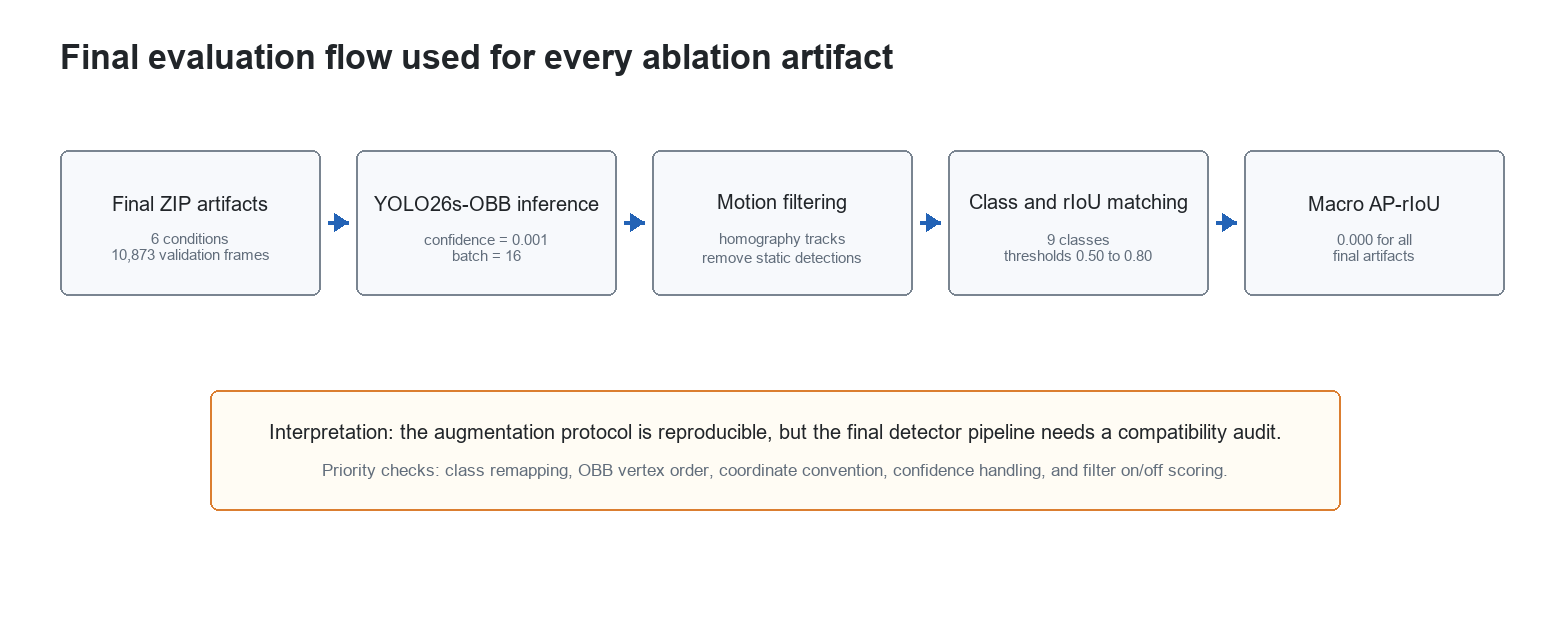
\includegraphics[width=0.93\textwidth]{latex_report/src/fig/final_evaluation_flow.png}
  \caption{Final evaluation flow applied to each ablation artifact. The same validation frames, prediction threshold, motion filter, class mapping, and rIoU thresholds are used for the six conditions.}
  \label{fig:final_evaluation_flow}
\end{figure*}

\subsubsection{Dataset and Augmentation Artifacts}
\label{sec:dataset_characterization_results}

The preprocessing audit confirms that the source training CSV contains 54,262 frames, 1,088 clips, and 601,934 oriented-box annotations. The validation subset used by the final evaluator contains 10,873 frames and 109,448 ground-truth instances, which means that the reported detector results are measured on a fixed validation partition rather than on synthetic or resampled validation data.

The train-only augmentation release, named SAM CP production v1, contains 1,501 synthetic images and 1,501 matching YOLO-OBB label files, with 3,391 inserted vehicle instances. No synthetic validation files are generated. This is important because the ablation is designed to test whether synthetic training evidence helps the model, not whether synthetic examples leak into the validation set. Table~\ref{tab:augmentation_release_summary} summarizes the generated augmentation set.

\begin{table}[!t]
  \caption{SAM copy-paste augmentation set used for training.}
  \label{tab:augmentation_release_summary}
  \centering
  \small
  \begin{tabular}{@{}p{0.60\columnwidth}p{0.32\columnwidth}@{}}
    \toprule
    \textbf{Indicator} & \textbf{Value} \\
    \midrule
    Run ID & SAM CP production v1 \\
    Synthetic images & 1,501 \\
    Synthetic label files & 1,501 \\
    Inserted instances & 3,391 \\
    Validation files generated & 0 \\
    Kernel elapsed time & 652.35 s \\
    Peak GPU memory & 3,297 MiB \\
    Peak GPU utilization & 99\% \\
    \bottomrule
  \end{tabular}
\end{table}

The validation checks cover the main failure modes that could compromise the augmentation release: image-label stem mismatches, empty deltas, malformed YOLO-OBB labels, out-of-range coordinates, synthetic files that shadow real frames, and synthetic backgrounds taken from outside the train split. These checks support the reproducibility of the augmentation process. However, they do not by themselves prove that the generated data improves the detector; that claim must come from the final evaluator.

\subsubsection{Ablation Artifact Status}
\label{sec:ablation_artifact_status}

Table~\ref{tab:ablation_artifact_status} records the final artifact used for each experimental condition. Since every condition is represented by a final evaluator ZIP, the six runs can be compared under the same final metric schema.

\begin{table*}[!t]
  \caption{Final ablation artifacts available for analysis.}
  \label{tab:ablation_artifact_status}
  \centering
  \small
  \begin{tabular}{p{0.14\textwidth} p{0.27\textwidth} p{0.22\textwidth} p{0.27\textwidth}}
    \toprule
    \textbf{Condition} & \textbf{Role in the ablation} & \textbf{Final weight} & \textbf{Artifact interpretation} \\
    \midrule
    Base 0 & Zero-shot YOLO26s-OBB with DOTA vehicle mapping & \texttt{yolo26s-obb.pt} & Final evaluator ZIP; reference without task-specific training \\
    Base 1 & Raw-data baseline with minimal online augmentation & \texttt{f1\_c1\_best.pt} & Final evaluator ZIP; raw trained baseline \\
    Base 2 & Raw-data baseline with stronger classical YOLO augmentation & \texttt{f1\_c2\_best.pt} & Final evaluator ZIP; classical augmentation baseline \\
    Improvement A & LaMa-corrected training pixels with minimal profile & \texttt{f1\_c3\_best.pt} & Final evaluator ZIP; pixel-correction ablation \\
    Improvement B & Raw pixels plus train-only SAM copy-paste delta & \texttt{f1\_mejora\_b\_best.pt} & Final evaluator ZIP plus internal training logs \\
    Improvement C & LaMa-corrected pixels plus the same SAM copy-paste delta & \texttt{f1\_mejora\_c\_best.pt} & Final evaluator ZIP; combined pixel-correction and copy-paste ablation \\
    \bottomrule
  \end{tabular}
\end{table*}

\subsubsection{Final Macro AP-rIoU Comparison}
\label{sec:final_macro_ap_results}

Table~\ref{tab:ablation_final_metrics} and Figure~\ref{fig:ablation_macro_metrics} show the central result of the final artifact set: every condition obtains 0.000 Macro AP-rIoU, 0.000 AP@0.50, and 0.000 AP@0.80. This includes the raw trained baseline, the classical augmentation baseline, the LaMa-only condition, and both SAM copy-paste conditions. The result is therefore not a small performance difference among methods; it is a complete failure to produce accepted true positives under the final class-and-rotated-geometry matcher.

The count snapshot at rIoU 0.50 confirms the same conclusion. The true-positive count is zero for all conditions, while the false-negative count remains 109,448, equal to the number of validation ground-truth instances. Since rIoU 0.50 is the least strict threshold reported in the final metric, the zero result at this threshold implies that the failure is already present before the stricter 0.55--0.80 thresholds are applied.

\begin{table*}[!t]
  \caption{Final ablation metrics. Counts are reported at rIoU 0.50 after motion filtering.}
  \label{tab:ablation_final_metrics}
  \centering
  \scriptsize
  \resizebox{\textwidth}{!}{%
  \begin{tabular}{p{0.14\textwidth} c c c p{0.23\textwidth} c c}
    \toprule
    \textbf{Condition} & \textbf{Macro AP-rIoU} & \textbf{AP@0.50} & \textbf{AP@0.80} & \textbf{TP / FP / FN @0.50} & \textbf{FPS} & \textbf{Mean inference} \\
    \midrule
    Base 0 & 0.000 & 0.000 & 0.000 & 0 / 319,557 / 109,448 & 38.9 & 16.87 ms \\
    Base 1 & 0.000 & 0.000 & 0.000 & 0 / 149,092 / 109,448 & 84.9 & 6.61 ms \\
    Base 2 & 0.000 & 0.000 & 0.000 & 0 / 252,890 / 109,448 & 85.5 & 6.30 ms \\
    Improvement A & 0.000 & 0.000 & 0.000 & 0 / 253,713 / 109,448 & 83.8 & 6.03 ms \\
    Improvement B & 0.000 & 0.000 & 0.000 & 0 / 261,587 / 109,448 & 90.2 & 5.71 ms \\
    Improvement C & 0.000 & 0.000 & 0.000 & 0 / 201,344 / 109,448 & 98.9 & 5.66 ms \\
    \bottomrule
  \end{tabular}
  }
\end{table*}

\begin{figure*}[!t]
  \centering
  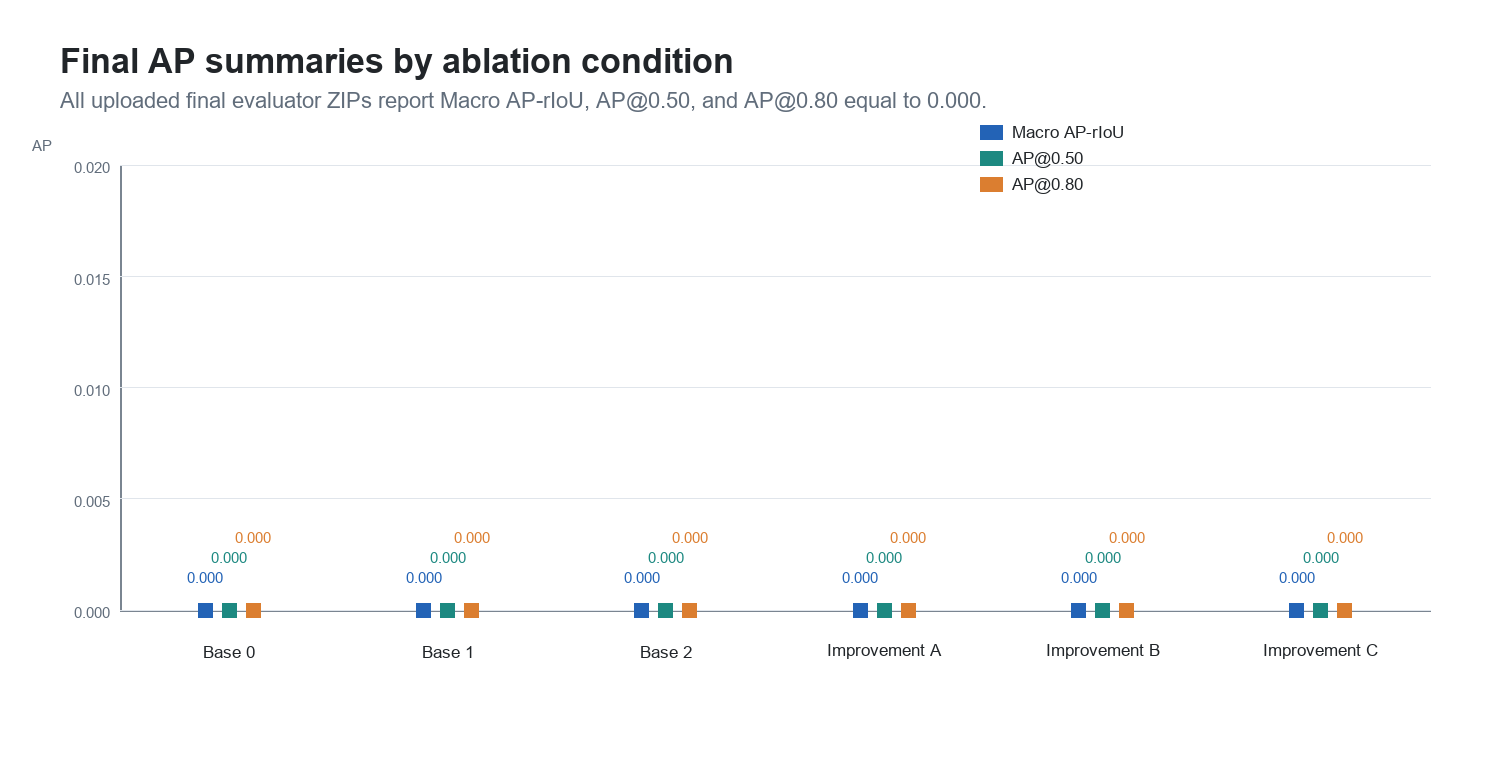
\includegraphics[width=0.90\textwidth]{latex_report/src/fig/ablation_macro_metrics.png}
  \caption{Final Macro AP-rIoU, AP@0.50, and AP@0.80 for the six final evaluator artifacts. All three AP summaries are 0.000 for every condition.}
  \label{fig:ablation_macro_metrics}
\end{figure*}

\begin{figure*}[!t]
  \centering
  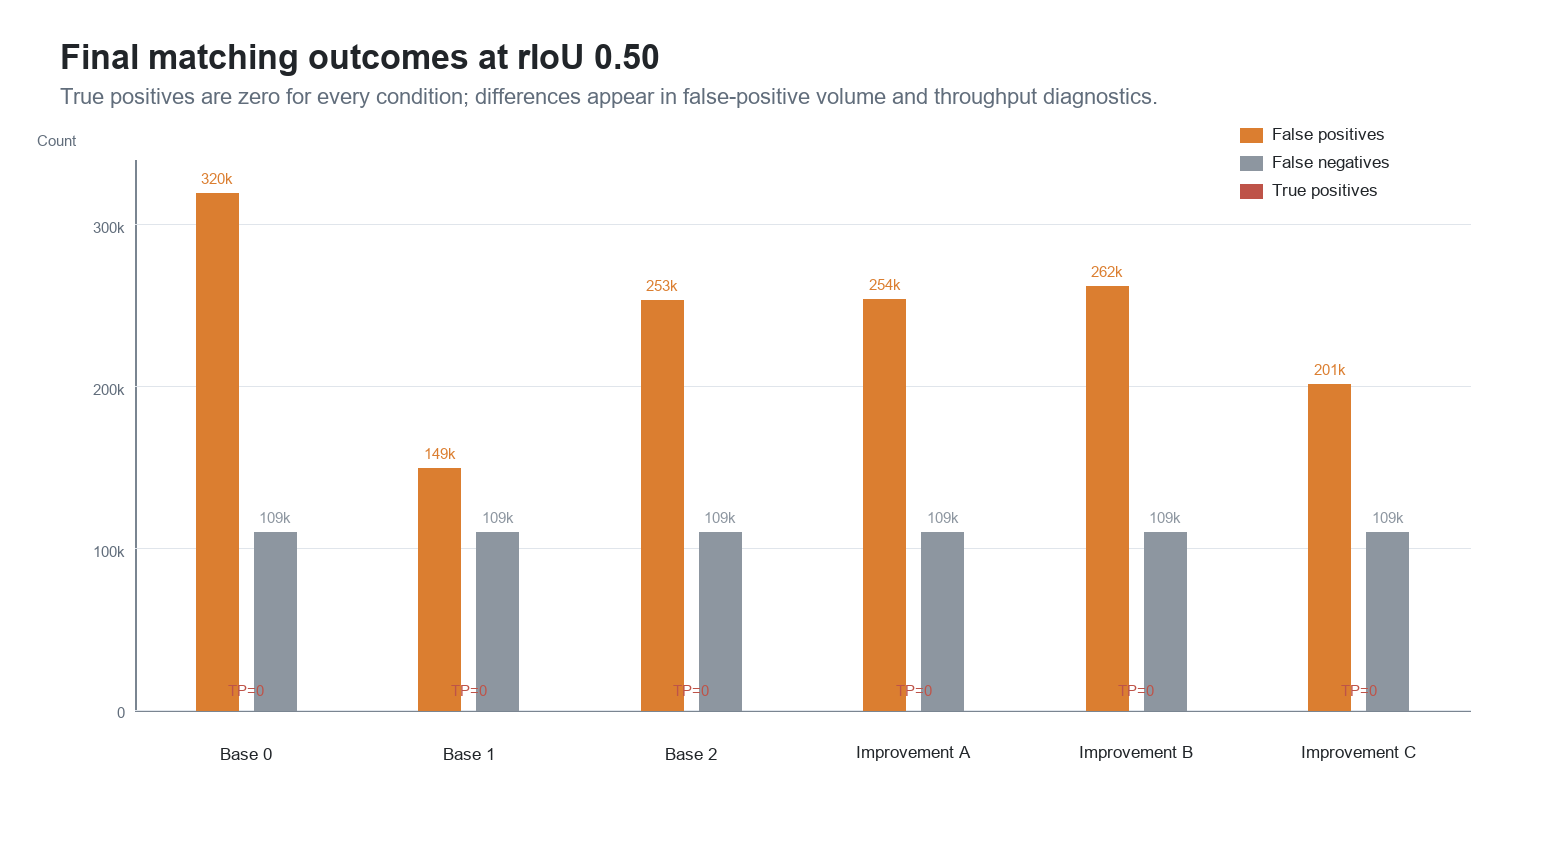
\includegraphics[width=0.92\textwidth]{latex_report/src/fig/ablation_outcomes_riou50.png}
  \caption{True positives, false positives, and false negatives at rIoU 0.50 after motion filtering. Every condition emits candidate detections, but none is accepted as a true positive by the final evaluator.}
  \label{fig:ablation_outcomes_riou50}
\end{figure*}

\subsubsection{Operational and Motion-Filter Diagnostics}
\label{sec:operational_diagnostics_results}

Although all AP values are zero, the artifacts are still informative because they show how each condition behaves before final matching. Figure~\ref{fig:ablation_fp_fps} compares false-positive volume and throughput. Base 0 is the slowest condition and has the highest false-positive count, which is consistent with a zero-shot model using only a partial DOTA-to-task class mapping. Base 1 has the lowest false-positive count among the trained conditions, with 149,092 false positives at rIoU 0.50, but it still has no true positives. Base 2, Improvement A, and Improvement B all increase the post-filter false-positive volume relative to Base 1.

Among the synthetic and LaMa-related variants, Improvement C has the best operational profile. It reduces false positives to 201,344, which is 20.4\% lower than Base 2, 20.7\% lower than Improvement A, and 23.0\% lower than Improvement B. It is also the fastest condition, reaching 98.9 FPS. This suggests that the LaMa plus SAM copy-paste setup changes the detector's candidate distribution in a useful operational direction. However, this cannot be reported as a detection-performance gain because the true-positive count remains zero and the final Macro AP-rIoU remains 0.000.

\begin{figure*}[!t]
  \centering
  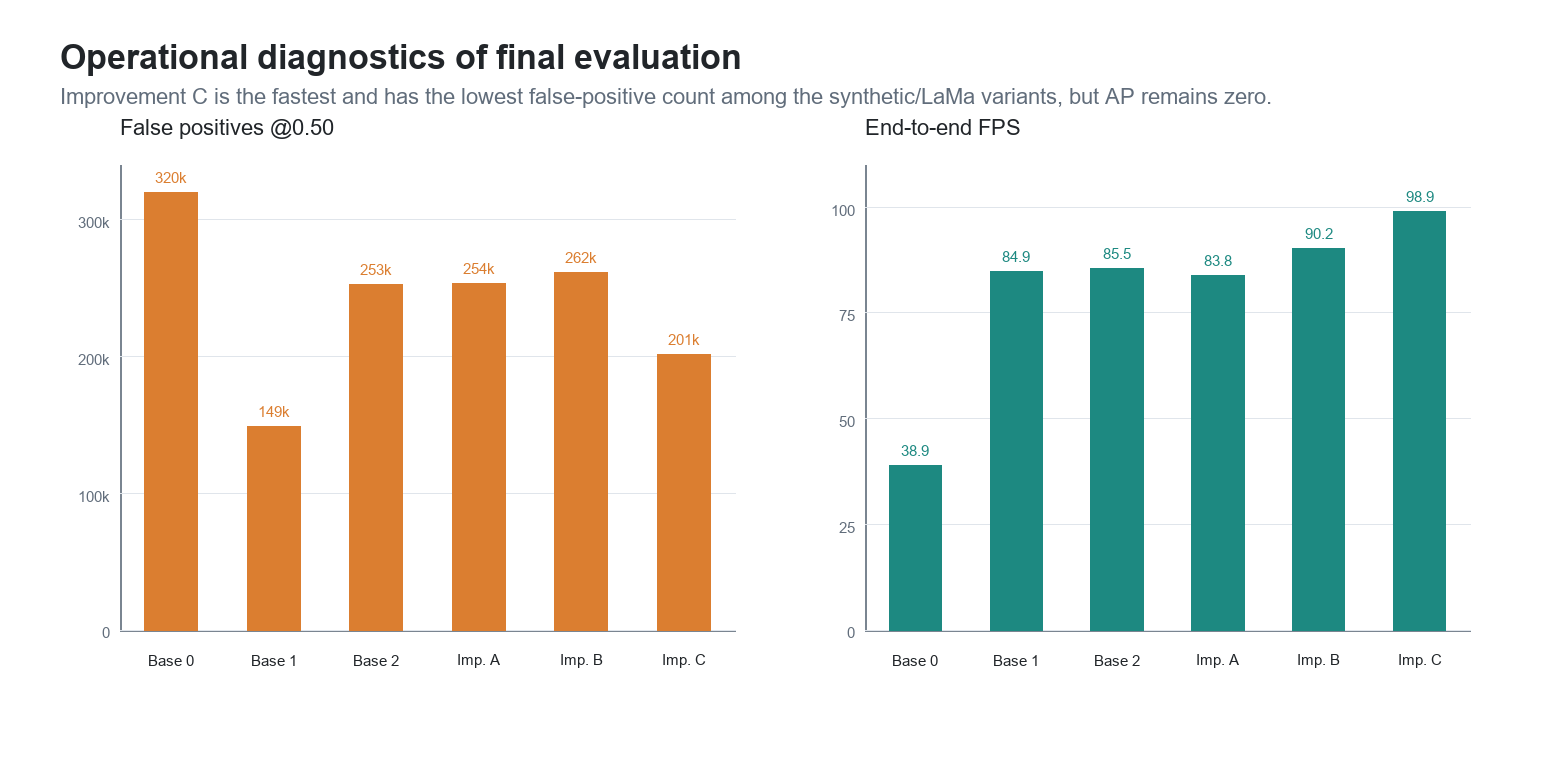
\includegraphics[width=0.92\textwidth]{latex_report/src/fig/ablation_fp_fps.png}
  \caption{Operational comparison of false-positive count and end-to-end throughput. Improvement C reduces false positives among the synthetic/LaMa variants and records the highest FPS, but the final AP score remains zero.}
  \label{fig:ablation_fp_fps}
\end{figure*}

The motion-filter diagnostics in Table~\ref{tab:motion_filter_diagnostics} also show that the evaluator is not simply discarding every prediction. The number of removed predictions varies by condition, from 43,172 in Base 1 to 306,852 in Base 0. The trained conditions form thousands of tracks, and the filter removes a subset identified as static. Therefore, the zero AP result should be interpreted as a final matching problem after filtering rather than as the absence of model output.

\begin{table*}[!t]
  \caption{Motion-filter and runtime diagnostics from the final evaluator artifacts.}
  \label{tab:motion_filter_diagnostics}
  \centering
  \scriptsize
  \resizebox{\textwidth}{!}{%
  \begin{tabular}{p{0.16\textwidth} r r r r r}
    \toprule
    \textbf{Condition} & \textbf{Removed predictions} & \textbf{Static tracks} & \textbf{Total tracks} & \textbf{Elapsed time} & \textbf{FPS} \\
    \midrule
    Base 0 & 306,852 & 9,120 & 56,619 & 279.7 s & 38.9 \\
    Base 1 & 43,172 & 1,539 & 23,385 & 128.1 s & 84.9 \\
    Base 2 & 81,956 & 3,466 & 58,591 & 127.2 s & 85.5 \\
    Improvement A & 100,053 & 3,827 & 51,784 & 129.8 s & 83.8 \\
    Improvement B & 101,569 & 4,122 & 51,392 & 120.6 s & 90.2 \\
    Improvement C & 78,594 & 3,043 & 39,144 & 109.9 s & 98.9 \\
    \bottomrule
  \end{tabular}
  }
\end{table*}

\subsubsection{Class-Level Error Distribution}
\label{sec:class_error_distribution_results}

Because no condition obtains non-zero AP, class-level AP cannot be used to identify strong classes. The useful class-level evidence is instead the distribution of false positives at rIoU 0.50, shown in Figure~\ref{fig:class_fp_by_condition}. Auto dominates the false-positive volume in every trained condition, which is expected because it is the majority class in the dataset. Motocicleta is the second major source of unmatched detections for Base 1, Base 2, Improvement A, and Improvement B. Improvement C reduces Motocicleta false positives to 67,510, compared with 120,836 in Improvement B and 114,589 in Improvement A, but it still does not recover any true positive under the final evaluator.

The heatmap also clarifies the role of Base 0. Its predictions are concentrated in Auto and Camion because the zero-shot DOTA mapping only connects the pretrained vehicle categories to those official task classes. This makes Base 0 useful as a sanity reference for zero-shot inference, but not as a complete nine-class trained model.

\begin{figure*}[!t]
  \centering
  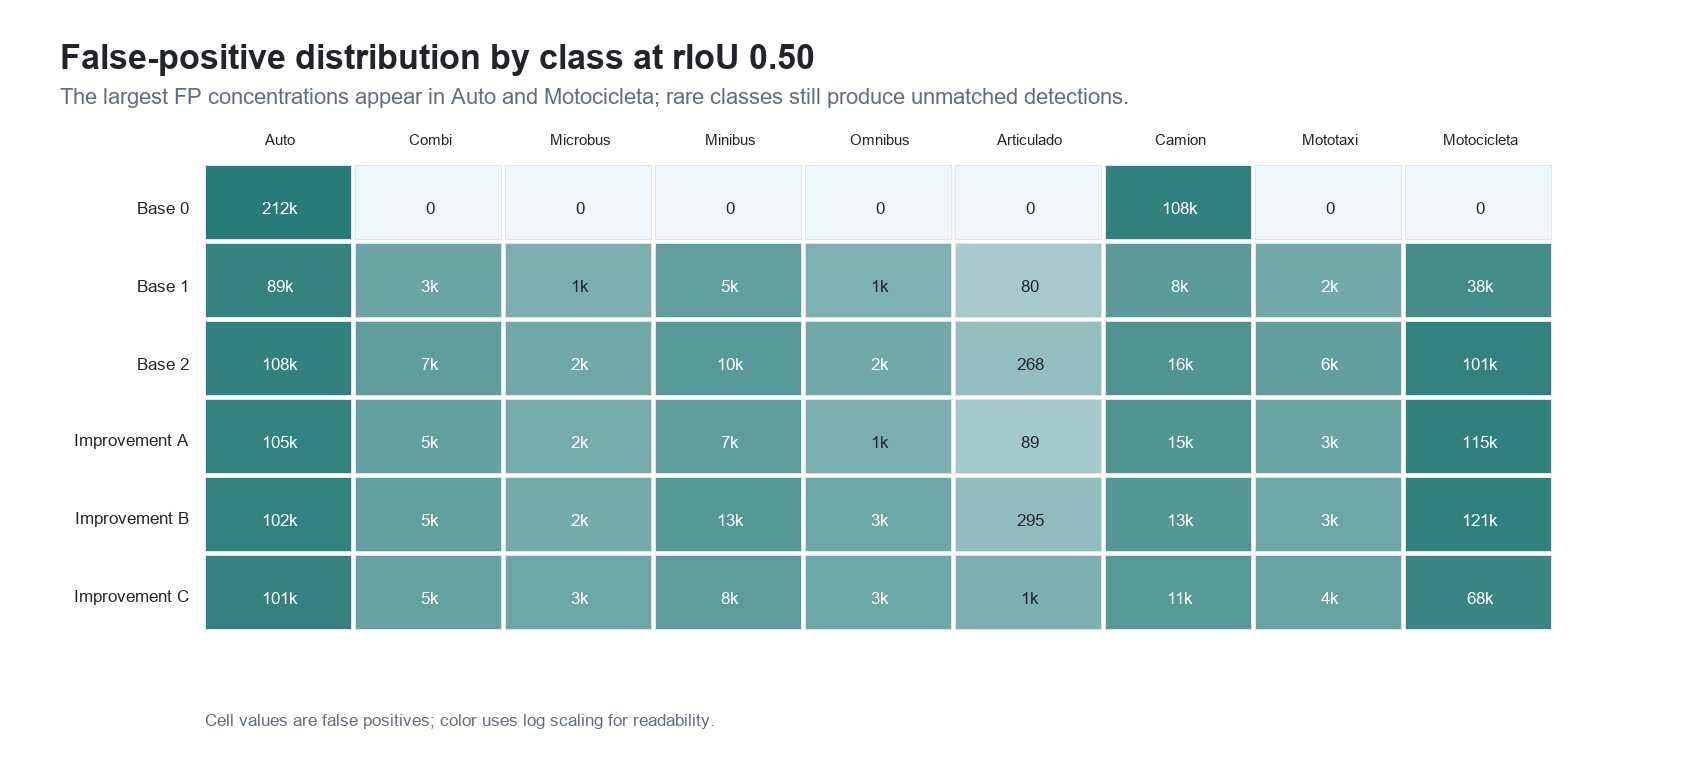
\includegraphics[width=0.95\textwidth]{latex_report/src/fig/class_fp_by_condition.png}
  \caption{False-positive distribution by class at rIoU 0.50. Values are post-filter false positives; color intensity is log-scaled for readability.}
  \label{fig:class_fp_by_condition}
\end{figure*}

\subsubsection{Improvement B Internal Training Evidence}
\label{sec:improvement_b_training_results}

Improvement B now has a final evaluator ZIP, but its training artifacts remain useful because they expose a sharp discrepancy between internal validation and final scoring. The uploaded run completed 12 epochs of a requested 40-epoch schedule with patience 5, batch size 96, image size 640, AdamW, automatic mixed precision, and two Tesla T4 GPUs. The best internal Ultralytics validation mAP50 is 0.929 at epoch 11, and the best internal mAP50-95 is 0.761 at epoch 7. The last recorded epoch reports precision 0.900, recall 0.859, mAP50 0.928, and mAP50-95 0.757.

\begin{figure*}[!t]
  \centering
  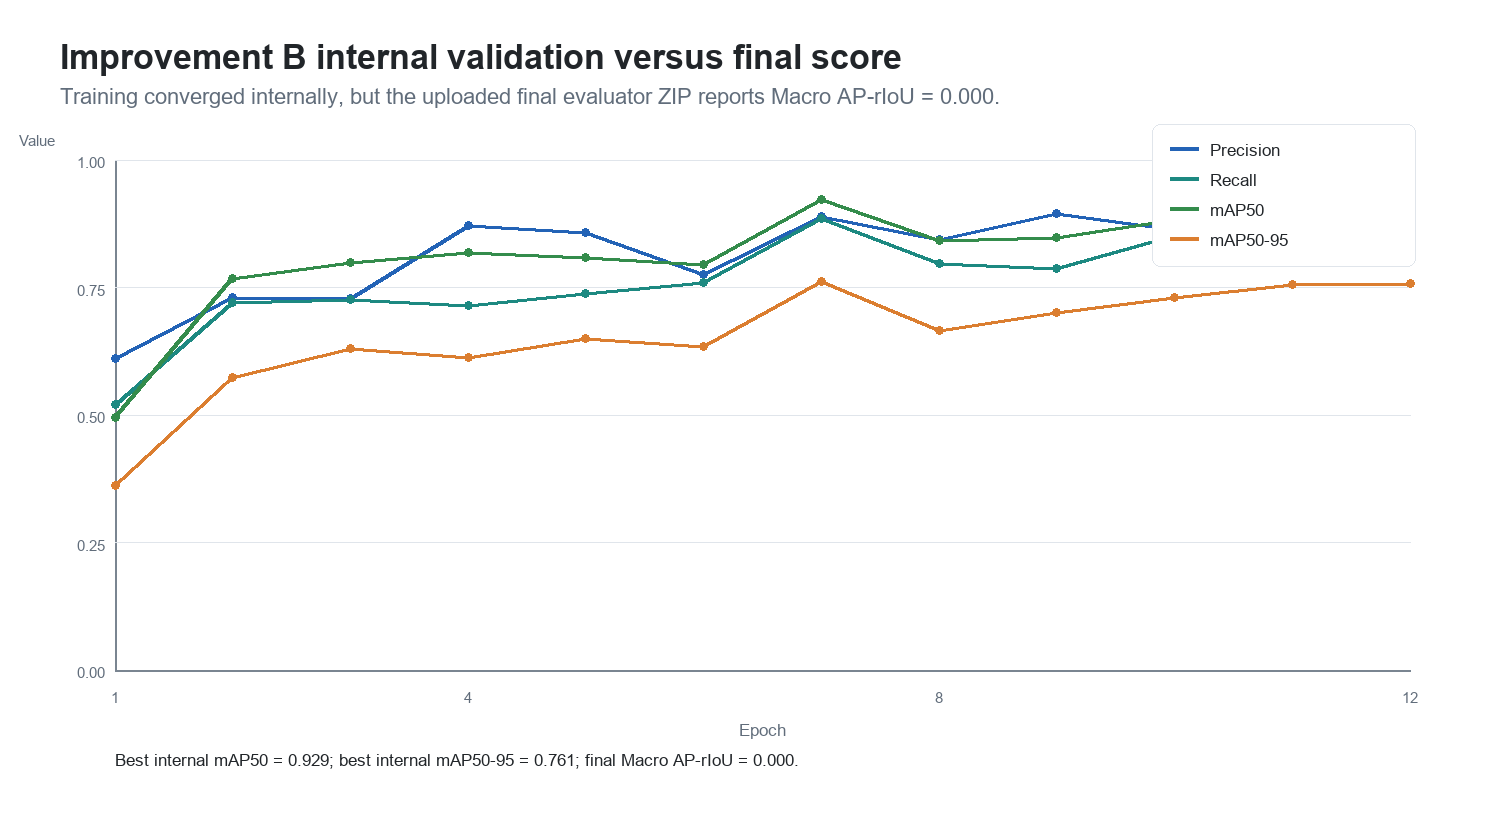
\includegraphics[width=0.90\textwidth]{latex_report/src/fig/mejora_b_training_curves.png}
  \caption{Internal Ultralytics validation curves for Improvement B. The run converges internally, but the final Macro AP-rIoU evaluator reports 0.000 for the same condition.}
  \label{fig:mejora_b_training_curves}
\end{figure*}

This discrepancy is one of the most important diagnostic findings of the study. Ultralytics validation and the paper's final evaluator are not identical measurements: the final score uses the SMART validation frames, official class identifiers, rotated-IoU thresholds, homography-based motion filtering, and the final class-and-geometry matching implementation. Therefore, the high internal mAP of Improvement B cannot be interpreted as evidence of final detector improvement. Instead, it indicates that the next technical priority is to audit the boundary between training validation outputs and final evaluator inputs.

\subsubsection{Summary of Key Findings}
\label{sec:key_findings_results}

Table~\ref{tab:key_findings} summarizes the main findings. The ablation does not support the hypothesis that the current SAM copy-paste release improves final Macro AP-rIoU. It does, however, produce a useful negative result: the augmentation pipeline is reproducible, all final artifacts are now available, and the final evaluator exposes a systematic mismatch that must be resolved before model-quality conclusions can be strengthened.

\begin{table*}[!t]
  \caption{Key findings from the completed final-artifact analysis.}
  \label{tab:key_findings}
  \centering
  \small
  \begin{tabular}{p{0.25\textwidth} p{0.33\textwidth} p{0.34\textwidth}}
    \toprule
    \textbf{Finding} & \textbf{Evidence} & \textbf{Interpretation} \\
    \midrule
    All final AP summaries are zero & Six final evaluator ZIPs report 0.000 Macro AP-rIoU, 0.000 AP@0.50, and 0.000 AP@0.80. & No condition can be claimed as the strongest detector under the current final metric. \\
    Candidate detections are present & False positives range from 149,092 to 319,557 at rIoU 0.50. & The failure occurs at final matching after prediction and filtering, not because models emit no boxes. \\
    Improvement C has the best operational profile among synthetic variants & 201,344 false positives and 98.9 FPS. & It improves candidate volume and speed relative to Base 2, Improvement A, and Improvement B, but not final AP. \\
    Improvement B has a training-final mismatch & Internal mAP50 reaches 0.929, while final Macro AP-rIoU is 0.000. & Training-loop validation is not a substitute for the paper's final evaluator. \\
    The next step is a compatibility audit & Zero true positives appear even at rIoU 0.50. & Class remapping, OBB vertex order, coordinate convention, confidence handling, and motion-filter effects must be checked. \\
    \bottomrule
  \end{tabular}
\end{table*}
